\documentclass{beamer}
\mode<presentation>{\usetheme{Madrid}}

\usepackage[utf8]{inputenc}
% Allows including images.
\usepackage{graphicx}

\title[Linux containers]{Linux containers}

\author{Bruno Barcarol Guimarães}
\institute[]{\textit{bbgstb@gmail.com}}
\date{2014-12-06}

\begin{document}

\begin{frame}
    \titlepage
\end{frame}

\begin{frame}
    \frametitle{Resumo}
    \tableofcontents
\end{frame}

\section{Visão geral}

\subsection{Tecnologias}

\begin{frame}
    \frametitle{Visão geral - Container}
    Container
    \begin{itemize}
        \item um grupo de processos
        \item sobre um mesmo \textit{kernel}
        \item isolado dos outros processos
    \end{itemize}
\end{frame}

\begin{frame}
    \frametitle{Visão geral - Tecnologias}
    \centering
    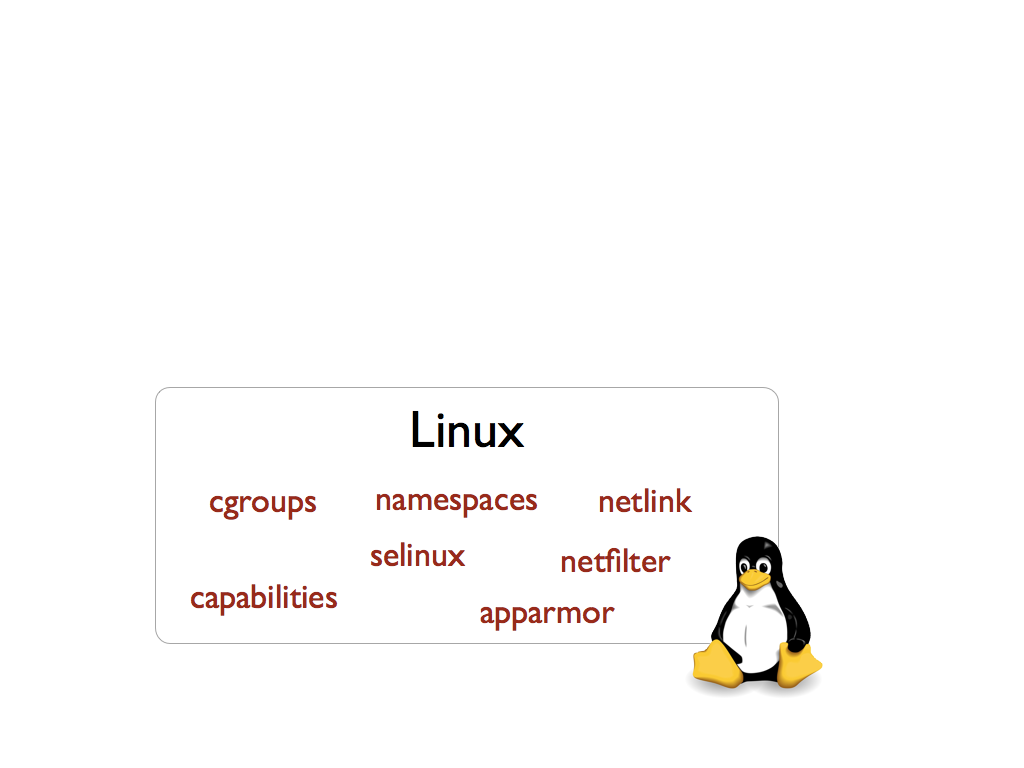
\includegraphics[width=1\linewidth]{img/docker_diagram_kernel.png}
\end{frame}

\begin{frame}
    \frametitle{Visão geral - Tecnologias}
    \centering
    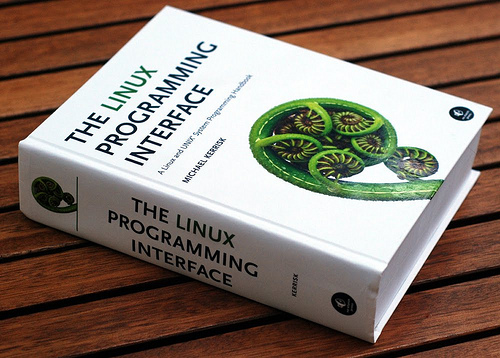
\includegraphics[width=0.8\linewidth]{img/the-linux-programming-interface.jpg}
\end{frame}

\begin{frame}
    \frametitle{Visão geral - Tecnologias}
    \centering
    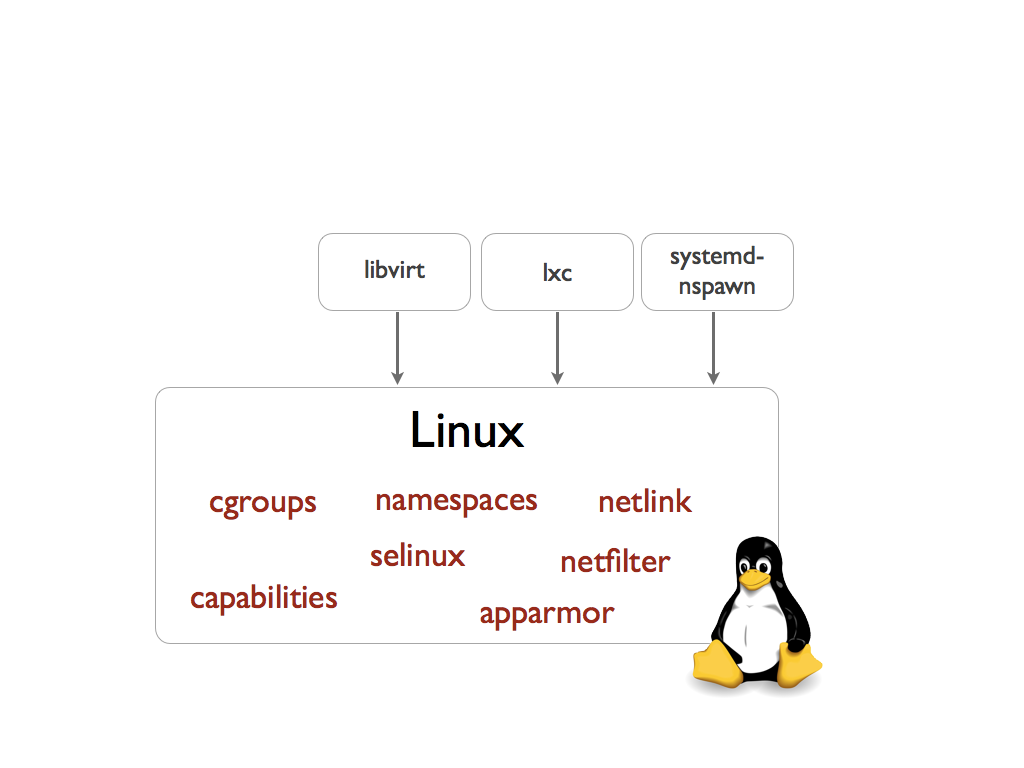
\includegraphics[width=1\linewidth]{img/docker_diagram_lxc.png}
\end{frame}

\begin{frame}
    \frametitle{Visão geral - Tecnologias}
    \centering
    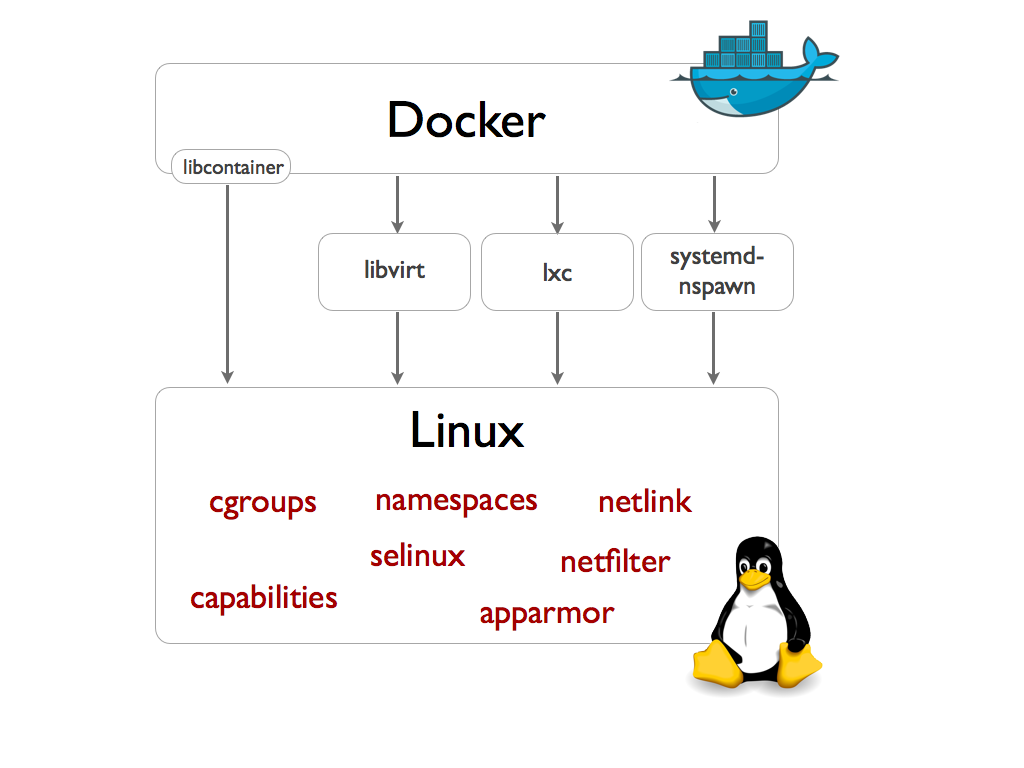
\includegraphics[width=1\linewidth]{img/docker-execdriver-diagram.png}
\end{frame}

\begin{frame}
    \frametitle{Visão geral - Tecnologias}
    \centering
    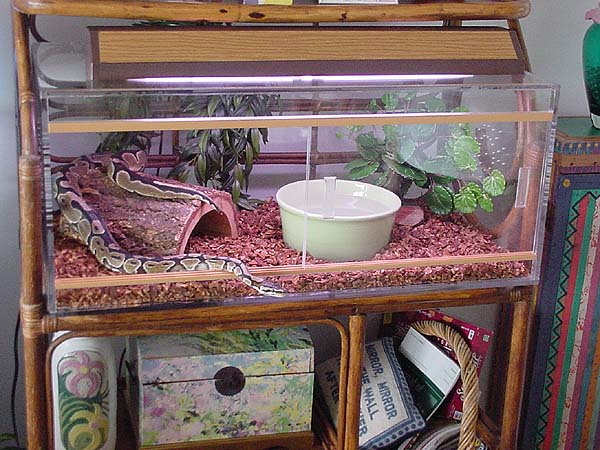
\includegraphics[width=0.8\linewidth]{img/BetsyAcyrilcSnakeCage02.JPG}
\end{frame}

\begin{frame}
    \frametitle{Visão geral - Tecnologias}
    \centering
    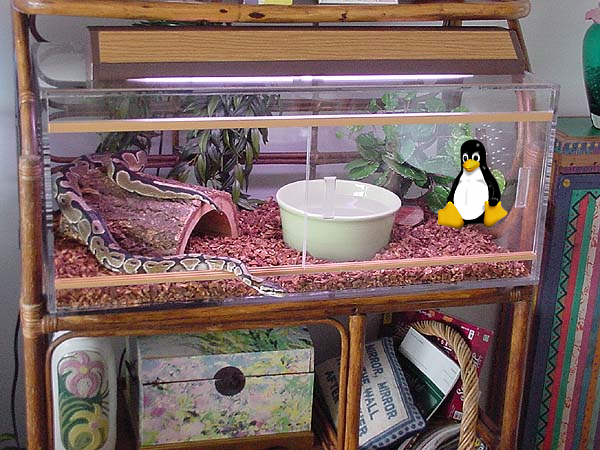
\includegraphics[width=0.8\linewidth]{img/BetsyAcyrilcSnakeCage02_tux.png}
\end{frame}

\begin{frame}
    \frametitle{Visão geral - Tecnologias}
    \centering
    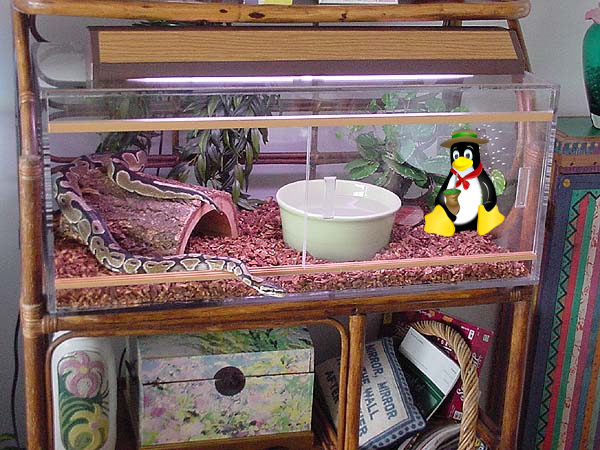
\includegraphics[width=0.8\linewidth]{img/BetsyAcyrilcSnakeCage02_tche_tux.png}
\end{frame}

\subsection{Vantagens e desvantages}

\begin{frame}
    \frametitle{Visão geral - Vantagens}
    \begin{itemize}
        \item \textit{kernel} compartilhado
            \begin{itemize}
                \item \textit{boot} mais rápido (\textit{ms})
                \item menor \textit{overhead}
                \item menor utlização de recursos
                \item uma única atualização
                    (\textit{kpatch}/\textit{ksplice}/\textit{live patching}?)
            \end{itemize}
    \end{itemize}
\end{frame}

\begin{frame}
    \frametitle{Visão geral - Desvantagens}
    \begin{itemize}
        \item \textit{kernel} compartilhado
        \begin{itemize}
            \item apenas um tipo (arquitetura, sistema operacional)
            \item apenas uma versão
            \item \textit{kernel exploits}
            \item segurança não era o objetivo principal
        \end{itemize}
    \end{itemize}
\end{frame}

\begin{frame}
    \frametitle{Visão geral}
    \centering
    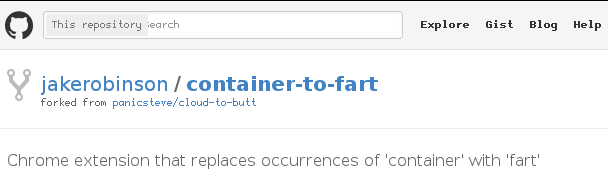
\includegraphics[width=0.8\linewidth]{img/chrome_extension.png}
\end{frame}

\section{Implementação}

\subsection{Kernel}

\begin{frame}
    \frametitle{Implementação - Kernel}
    \begin{itemize}
        \item cgroups
            \begin{itemize}
                \item limite/reserva de recursos
                \item \textit{accounting}
            \end{itemize}
        \item namespaces
            \begin{itemize}
                \item \texttt{clone(2)}
                \item \texttt{unshare(2)}
                \item \texttt{setns(2)}
            \end{itemize}
    \end{itemize}
\end{frame}

\subsection{Namespaces}

\begin{frame}
    \frametitle{Namespaces}
    \begin{itemize}
        \item mnt (\texttt{CLONE\_NEWNS})
        \item uts (\texttt{CLONE\_NEWUTS})
        \item ipc (\texttt{CLONE\_NEWIPC})
        \item pid (\texttt{CLONE\_NEWPID})
        \item net (\texttt{CLONE\_NEWNET})
        \item uid (\texttt{CLONE\_NEWUSER})
    \end{itemize}
\end{frame}

\begin{frame}
    \frametitle{Namespaces - mount}
    \begin{itemize}
        \item \texttt{CLONE\_NEWNS}
        \item linux 2.4.19
        \item \texttt{mount(2)/umount(2)}
        \item processos diferentes têm visões diferentes do sistema de arquivos
        \item ``\texttt{chroot(2)} \textit{on steroids}''
        \item compartilhamento de \textit{mount points}
    \end{itemize}
\end{frame}

\begin{frame}
    \frametitle{Namespaces - uts}
    \begin{itemize}
        \item \texttt{CLONE\_NEWUTS}
        \item linux 2.6.19
        \item \texttt{uname(2)}/\texttt{sethotname(2)}/\texttt{setdomainname(2)}
    \end{itemize}
\end{frame}

\begin{frame}
    \frametitle{Namespaces - ipc}
    \begin{itemize}
        \item \texttt{CLONE\_NEWIPC}
        \item linux 2.6.19 / linux 2.6.30
        \item \texttt{svipc(7)}/\texttt{mq\_overview(7)}
    \end{itemize}
\end{frame}

\begin{frame}
    \frametitle{Namespaces - pid}
    \begin{itemize}
        \item \texttt{CLONE\_NEWPID}
        \item linux 2.6.24
        \item processos em \textit{containers} diferentes podem ter o mesmo pid
        \item processos só vêem outros processos do mesmo \textit{namespace}
        \item migração entre \textit{hosts}
        \item múltiplos pid 1
        \item mapeamento de pid
        \item podem ser aninhados
    \end{itemize}
\end{frame}

\begin{frame}
    \frametitle{Namespaces - net}
    \begin{itemize}
        \item \texttt{CLONE\_NEWNET}
        \item linux 2.6.24
        \item cada \textit{namespace} tem seus próprios
            \begin{itemize}
                \item dispositivos de rede
                \item endereços ip
                \item tabelas de roteamento
                \item \texttt{/proc/net}
                \item portas
                \item etc
            \end{itemize}
    \end{itemize}
\end{frame}

\begin{frame}
    \frametitle{Namespaces - user}
    \begin{itemize}
        \item \texttt{CLONE\_NEWUSER}
        \item linux 2.6.23
        \item iniciado no kernel 2.6.23
        \item finalizado no kernel 3.8
        \item $\sim$ cinco anos
    \end{itemize}
\end{frame}

\begin{frame}
    \frametitle{Namespaces - user}
    \begin{itemize}
        \item isolamento de uid e gid
        \item mapeamento de uid e gid
        \item \texttt{uid 0}
    \end{itemize}
\end{frame}

\begin{frame}
    \frametitle{Namespaces - user}
    Recursivos
    \begin{itemize}
        \item um processo sem privilégios pode criar um \textit{namespace}
        \item \texttt{uid 0} dentro do \textit{namespace}
        \item ö
    \end{itemize}
\end{frame}

\section{Segurança}

\subsection{uid 0}

\begin{frame}
    \frametitle{Segurança - uid 0}
    \begin{itemize}
        \item não use
    \end{itemize}
\end{frame}

\subsection{Aplicações}

\begin{frame}
    \frametitle{Segurança - Aplicações}
    A maioria dos \textit{containers} executa uma tarefa específica, ao invés
    de um sistema completo, e a maioria dessas aplicações (apache, postgresql,
    mongodb, redis, ...) não precisa de privilégios de root. Os riscos são os
    mesmo que existiram até hoje: assumir que a aplicação pode fazer qualquer
    coisa para escapar do isolamento.
\end{frame}

\begin{frame}
    \frametitle{Segurança - Aplicações}
    syscalls
    \begin{itemize}
        \item e.g. \texttt{vmsplice(2)}
        \item limitar as \textit{syscalls} disponíveis
        \item seccomp/seccomp-bpf
        \item \textit{capabilities}
        \item grsec
        \item atualizações frequentes
    \end{itemize}
    = reduzir a área de exposição do kernel
\end{frame}

\begin{frame}
    \frametitle{Segurança - Aplicações}
    Outros \textit{containers}
    \begin{itemize}
        \item \textit{bug} no código dos \textit{namespaces}
        \item \textit{filesystem leak}
    \end{itemize}
\end{frame}

\begin{frame}
    \frametitle{Segurança - Aplicações}
    \begin{itemize}
        \item uid \textit{container} $->$ uid diferente no \textit{host}
        \item selinux
    \end{itemize}
\end{frame}

\begin{frame}
    \frametitle{Segurança}
    \begin{quote}
        ``[...] there's maybe marginal increases in practical security for
        certain kinds of deployment, and perhaps marginal decreases for others.
        We end up coming back to the attack surface, and it seems inevitable
        that that's always going to be larger in container environments. The
        question is, does it matter? If the larger attack surface still only
        results in one more vulnerability per thousand years, you probably
        don't care. The aim isn't to get containers to the same level of
        security as hypervisors, it's to get them close enough that the
        difference doesn't matter.''
    \end{quote}
    Matthew Garrett
\end{frame}

\section{Ferramentas}

\subsection{systemd-nspawn}

\begin{frame}
    \frametitle{systemd-nspawn}
\end{frame}

\subsection{lxc}

\begin{frame}
    \frametitle{lxc}
\end{frame}

\subsection{docker}

\begin{frame}
    \frametitle{docker}
\end{frame}

\section{Referências}

\begin{frame}
    \frametitle{Referências}
    \begin{itemize}
        \item
            \href
                {https://lwn.net/Articles/531114/}
                {Namespaces in operation}
        \item
            \href
                {http://mjg59.dreamwidth.org/33170.html}
                {Linux Container Security}
        \item
            \href
                {http://www.slideshare.net/jpetazzo/docker-linux-containers-lxc-and-security}
                {Docker, Linux Containers (LXC), and security}
        \item
            \href
                {https://lwn.net/Articles/268783/}
                {vmsplice(): the making of a local root exploit}
        \item
            \href
                {https://en.wikipedia.org/wiki/Seccomp}
                {seccomp}
        \item
            \href
                {https://en.wikipedia.org/wiki/Grsecurity}
                {grsec}
    \end{itemize}
\end{frame}

\begin{frame}
    \frametitle{Referências (imagens)}
    \begin{itemize}
        \item http://www.servicioswebgratis.com/wp-content/uploads/2012/08/the-linux-programming-interface.jpg
        \item http://www.mccarthyboas.com/BetsyAcyrilcSnakeCage02.JPG
        \item http://blog.docker.com/2014/03/docker-0-9-introducing-execution-drivers-and-libcontainer/
        \item http://tchelinux.org/media/tchelinux.svg
    \end{itemize}
\end{frame}

\end{document}
